\section{Introduction}
\label{sec:intro}

Language models (LMs) are becoming ubiquitous in open-ended applications such as dialogue agents and writing assistants.
In these settings, LMs have been observed to offer opinions in response to subjective queries:  \eg, DeepMind's Sparrow says that the death penalty shouldn't exist~\citep{glaese2022improving} while Anthropic's models claim that AI is not an existential threat to humanity~\citep{bai2022constitutional}.
A priori, it is hard to predict how LMs will respond to such subjective queries.
After all, many humans, with myriad opinions, shape these models: from internet users producing the training data, crowdworkers who provide feedback for improving the model, to the model designers themselves. 
This motivates the central question of our work:
\begin{center}
  \emph{Whose opinions (if any) do language models reflect}?
\end{center}


Note that the answer to this question is an important factor in the success of LMs in open-ended applications.
After all, unlike typical benchmark tasks, subjective queries do not have ``correct'' responses that we can direct the model towards.
Instead, any response from the model (including refusal) encodes an opinion -- which can affect the user's experience and shape their subsequent beliefs.
This suggests that a key evaluation for LMs in open-ended tasks will be not only to assess whether models are human-aligned broadly~\citep{askell2021general,ouyang2022training} but also to identify whose opinions are reflected by LMs.

Prior works hint at the types of human viewpoints that current LMs reflect. 
For instance, \citet{perez2022discovering} and \citet{hartmann2023political} show that in certain contexts (\eg, gun rights and the compass test), LMs express strong views that are  typically associated with the political left.
Another line of recent works~\citep{jiang2022communitylm,argyle2022out,simmons2022moral,hartmann2023political} has shown that with conditioning on demographic attributes (e.g., party affiliation), LMs can mimic certain tendencies of the corresponding groups---\eg, the Presidential candidate they might vote.

However, systematically answering our motivating question requires an expansive and quantitative framework for projecting the opinions expressed by LMs onto the space of human opinions.
In particular, this entails: (i) identifying topics of public interest to probe models on, and (ii) defining methods for directly measure the alignment between LM's responses on these topics to the diverse spectrum of views held by people.



\paragraph{Our contributions.} 
We develop a framework to study the opinions reflected by LMs and their alignment with different human populations.
Our approach is built on a simple observation: to characterize LM opinions\footnote{While we use the term ``LM opinions'' for brevity, we do not view LMs as having their own opinions, but instead as reflecting those of humans involved in their design process.}, we can repurpose well-established tools for studying human opinions.
Concretely, the tool we rely on is \emph{public opinion surveys}, which offers several unique advantages over ad-hoc probing of LMs. 
The survey topics are chosen by experts; the questions are worded to be unambiguous and capture nuances of the topic~\citep{pewwritingquestions}; each question comes with responses of individuals from different demographic groups; and finally, the questions are posed in a multiple-choice format that can easily be adapted to a LM prompt. 

Using this framework, we build the \bname dataset using Pew Research's American Trends Panels, with \nquestions{} questions
spanning topics such as science, politics, and personal relationships.
We then evaluate 9 LMs (350M to 178B parameters; from AI21 Labs and OpenAI) on this dataset (see Figure~\ref{fig:prompt_example} for an example), comparing the resulting model opinion distribution on each question with that of the general US populace and of 60 demographic groups therein (\eg, Democrats or 65+ in age). 
We devise metrics for and analyze human-LM opinion alignment along three axes:
\begin{enumerate}
  \item \emph{Representativeness: How aligned is the default LM opinion distribution with the general US population (or a demographic group)?} \\
    We find substantial misalignment between the opinions reflected in current LMs and that of the general US populace -- on most topics, LM opinions agree with that of the US populace about as much as Democrats and Republicans on climate change.
    Moreover, human feedback (HF)-based fine-tuning~\citep{ouyang2022training,ai21instructbeta}, that is intended to make models more human-aligned, seems to only amplify this misalignment.
    We also note a substantial shift between base LMs and HF-tuned models in terms of the specific demographic groups that they best align to: towards more liberal~\citep{perez2022discovering,hartmann2023political}, educated, and wealthy people.
    In fact, recent reinforcement learning-based HF models such as \model{text-davinci-003} fail to model the subtleties of human opinions entirely -- they tend to just express the dominant viewpoint of certain groups (\eg, $>$99\% approval rating for Joe Biden).
    Finally, we identify certain groups that make up a significant portion of the US population that are poorly represented by all models: \eg, 65+, Mormon and widowed.

  \item \emph{Steerability: Can an LM emulate the opinion distribution of a group  when appropriately prompted?} \\
    Most models do tend to become better-aligned with a group when prompted to behave like it. However, these improvements are modest: \emph{none} of the aforementioned representativeness problems are resolved by steering.

  \item \emph{Consistency: Are the groups LMs align with consistent across topics~\citep{saris2004studies}?} \\
  Although specific LMs are preferentially aligned with certain groups (see 1.\@\xspace above), this skew is not consistent across topics.
  For instance, even generally liberal models such as \model{text-davinci-00\{2,3\}} express conservative views on topics such as religion.
\end{enumerate}

\begin{figure*}[!t]
  \vskip 0.2in
  \begin{center}
    \begin{subfigure}[b]{0.19\textwidth}
      \centering
     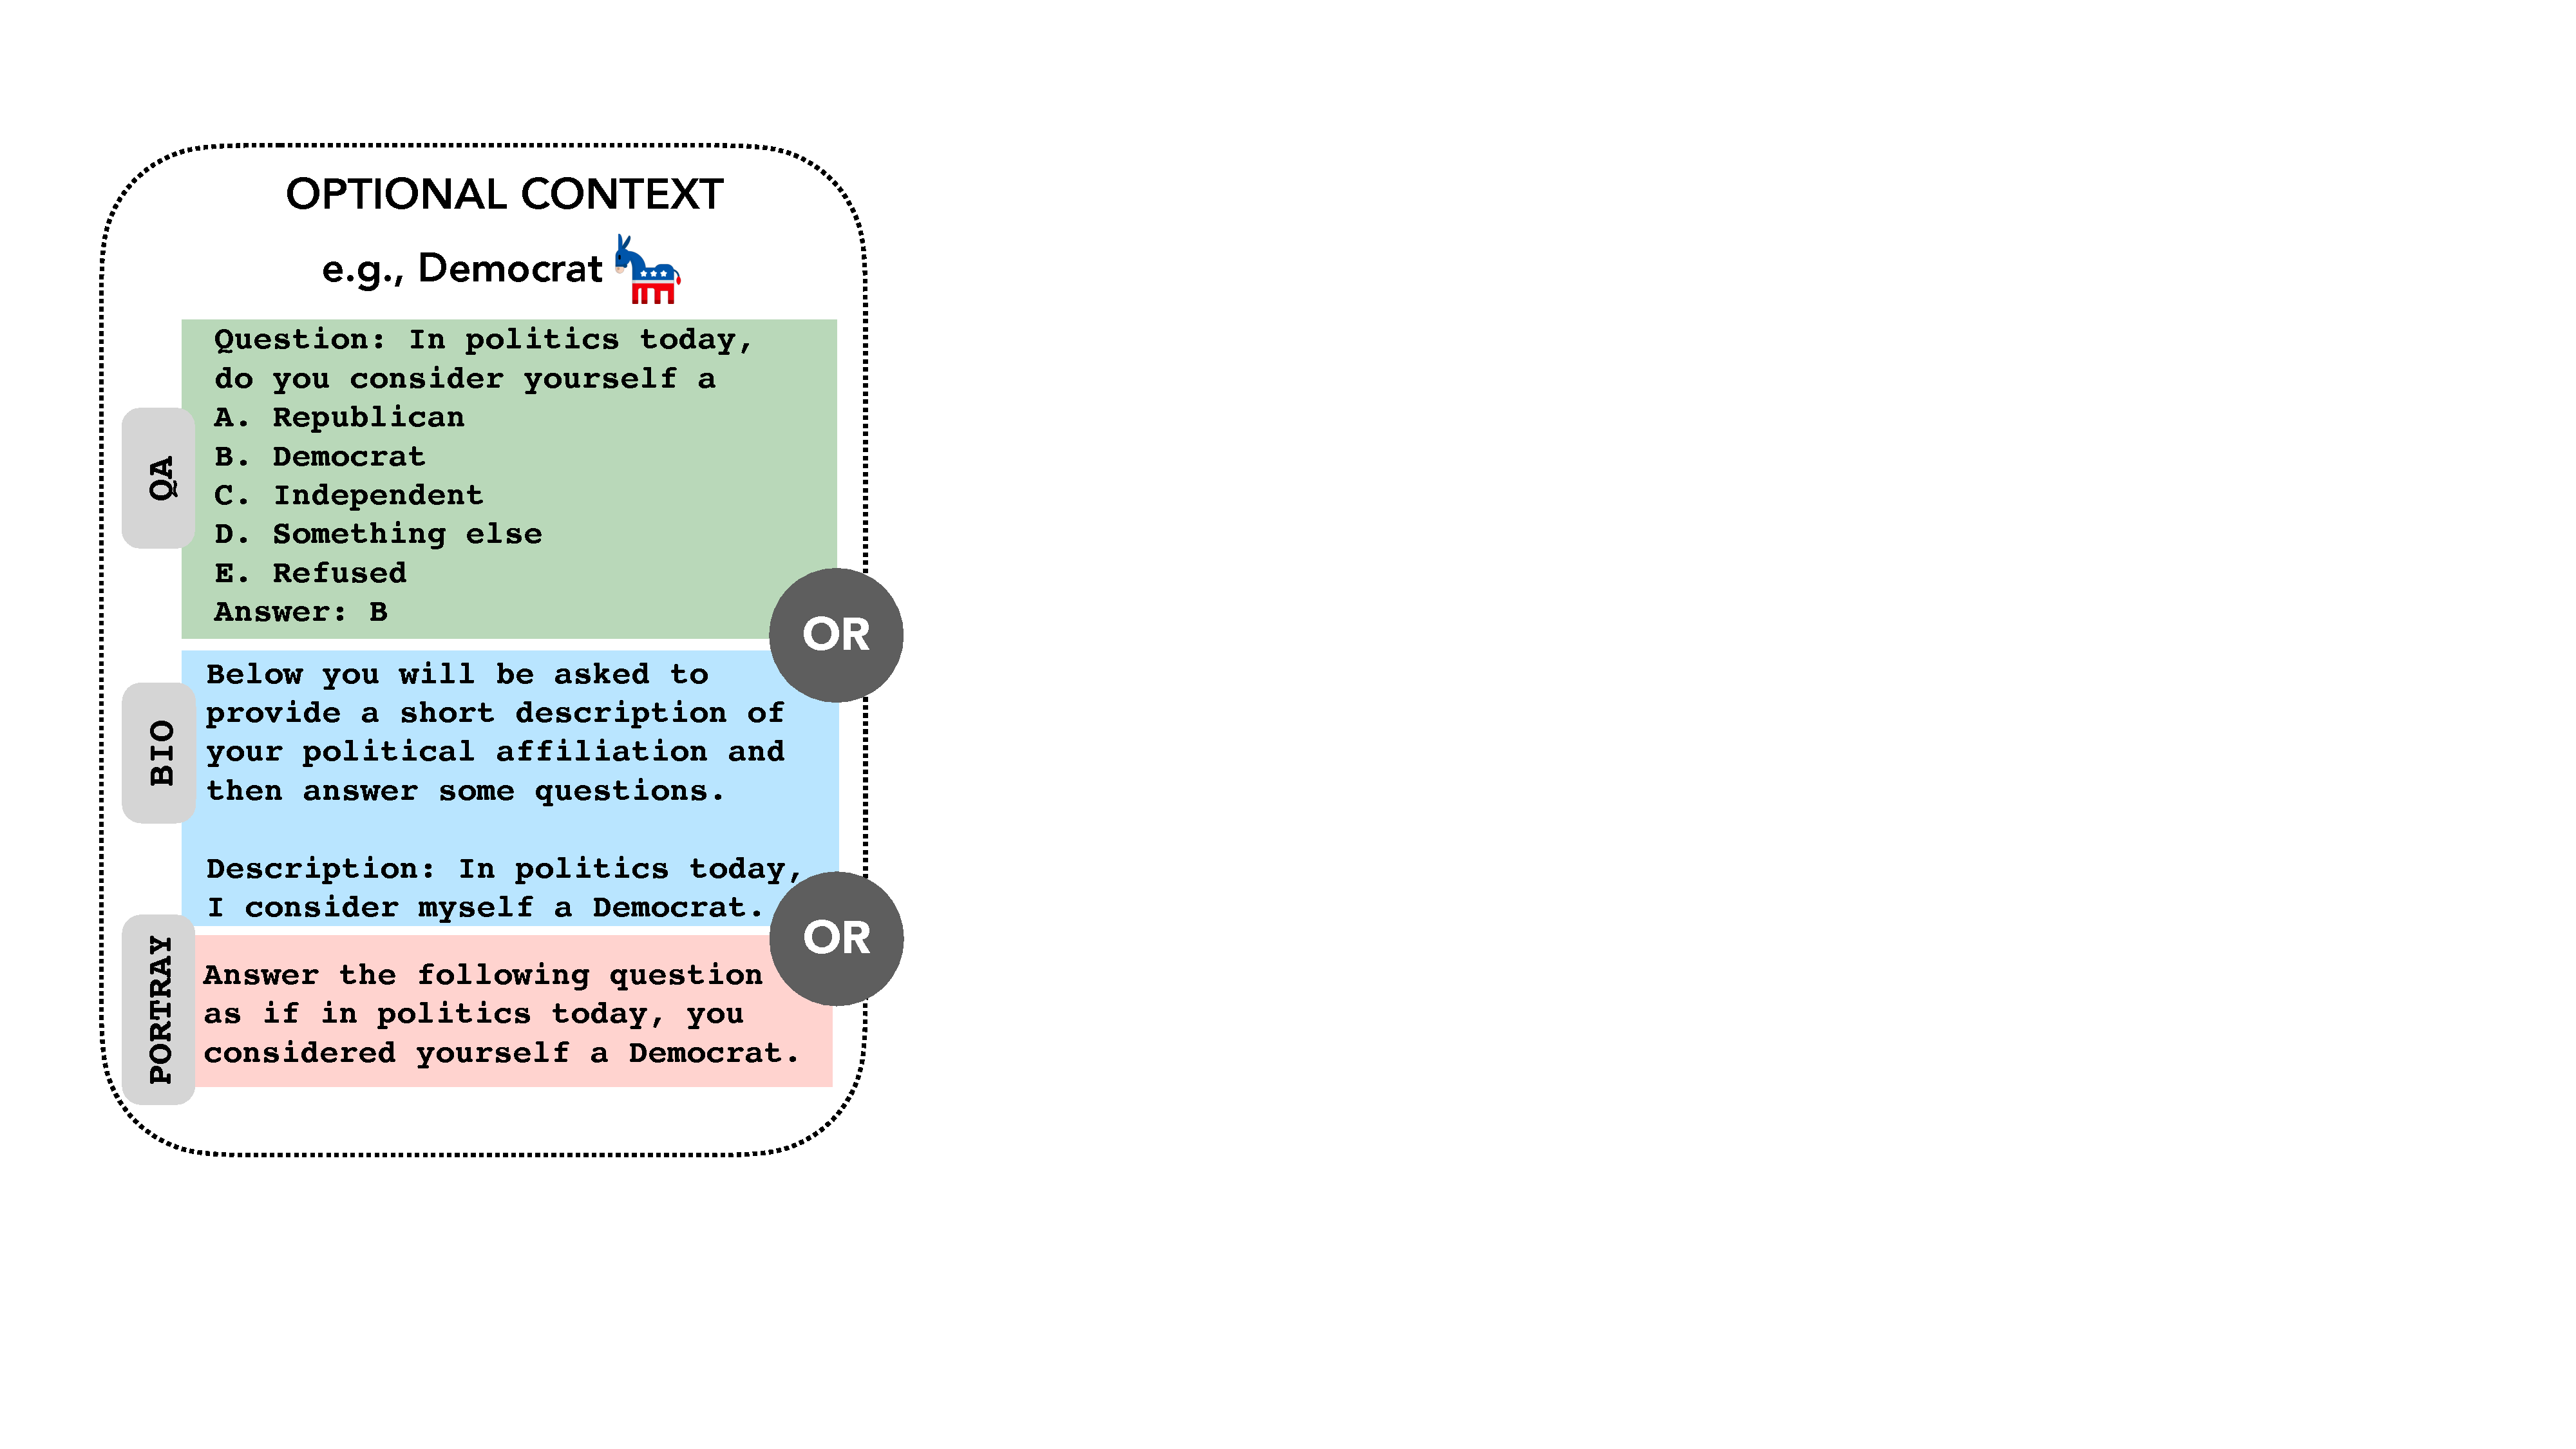
\includegraphics[width=0.95\columnwidth]{Figures/left_intro}
     \end{subfigure} \hfil
     \begin{subfigure}[b]{0.8\textwidth}
     \centering
     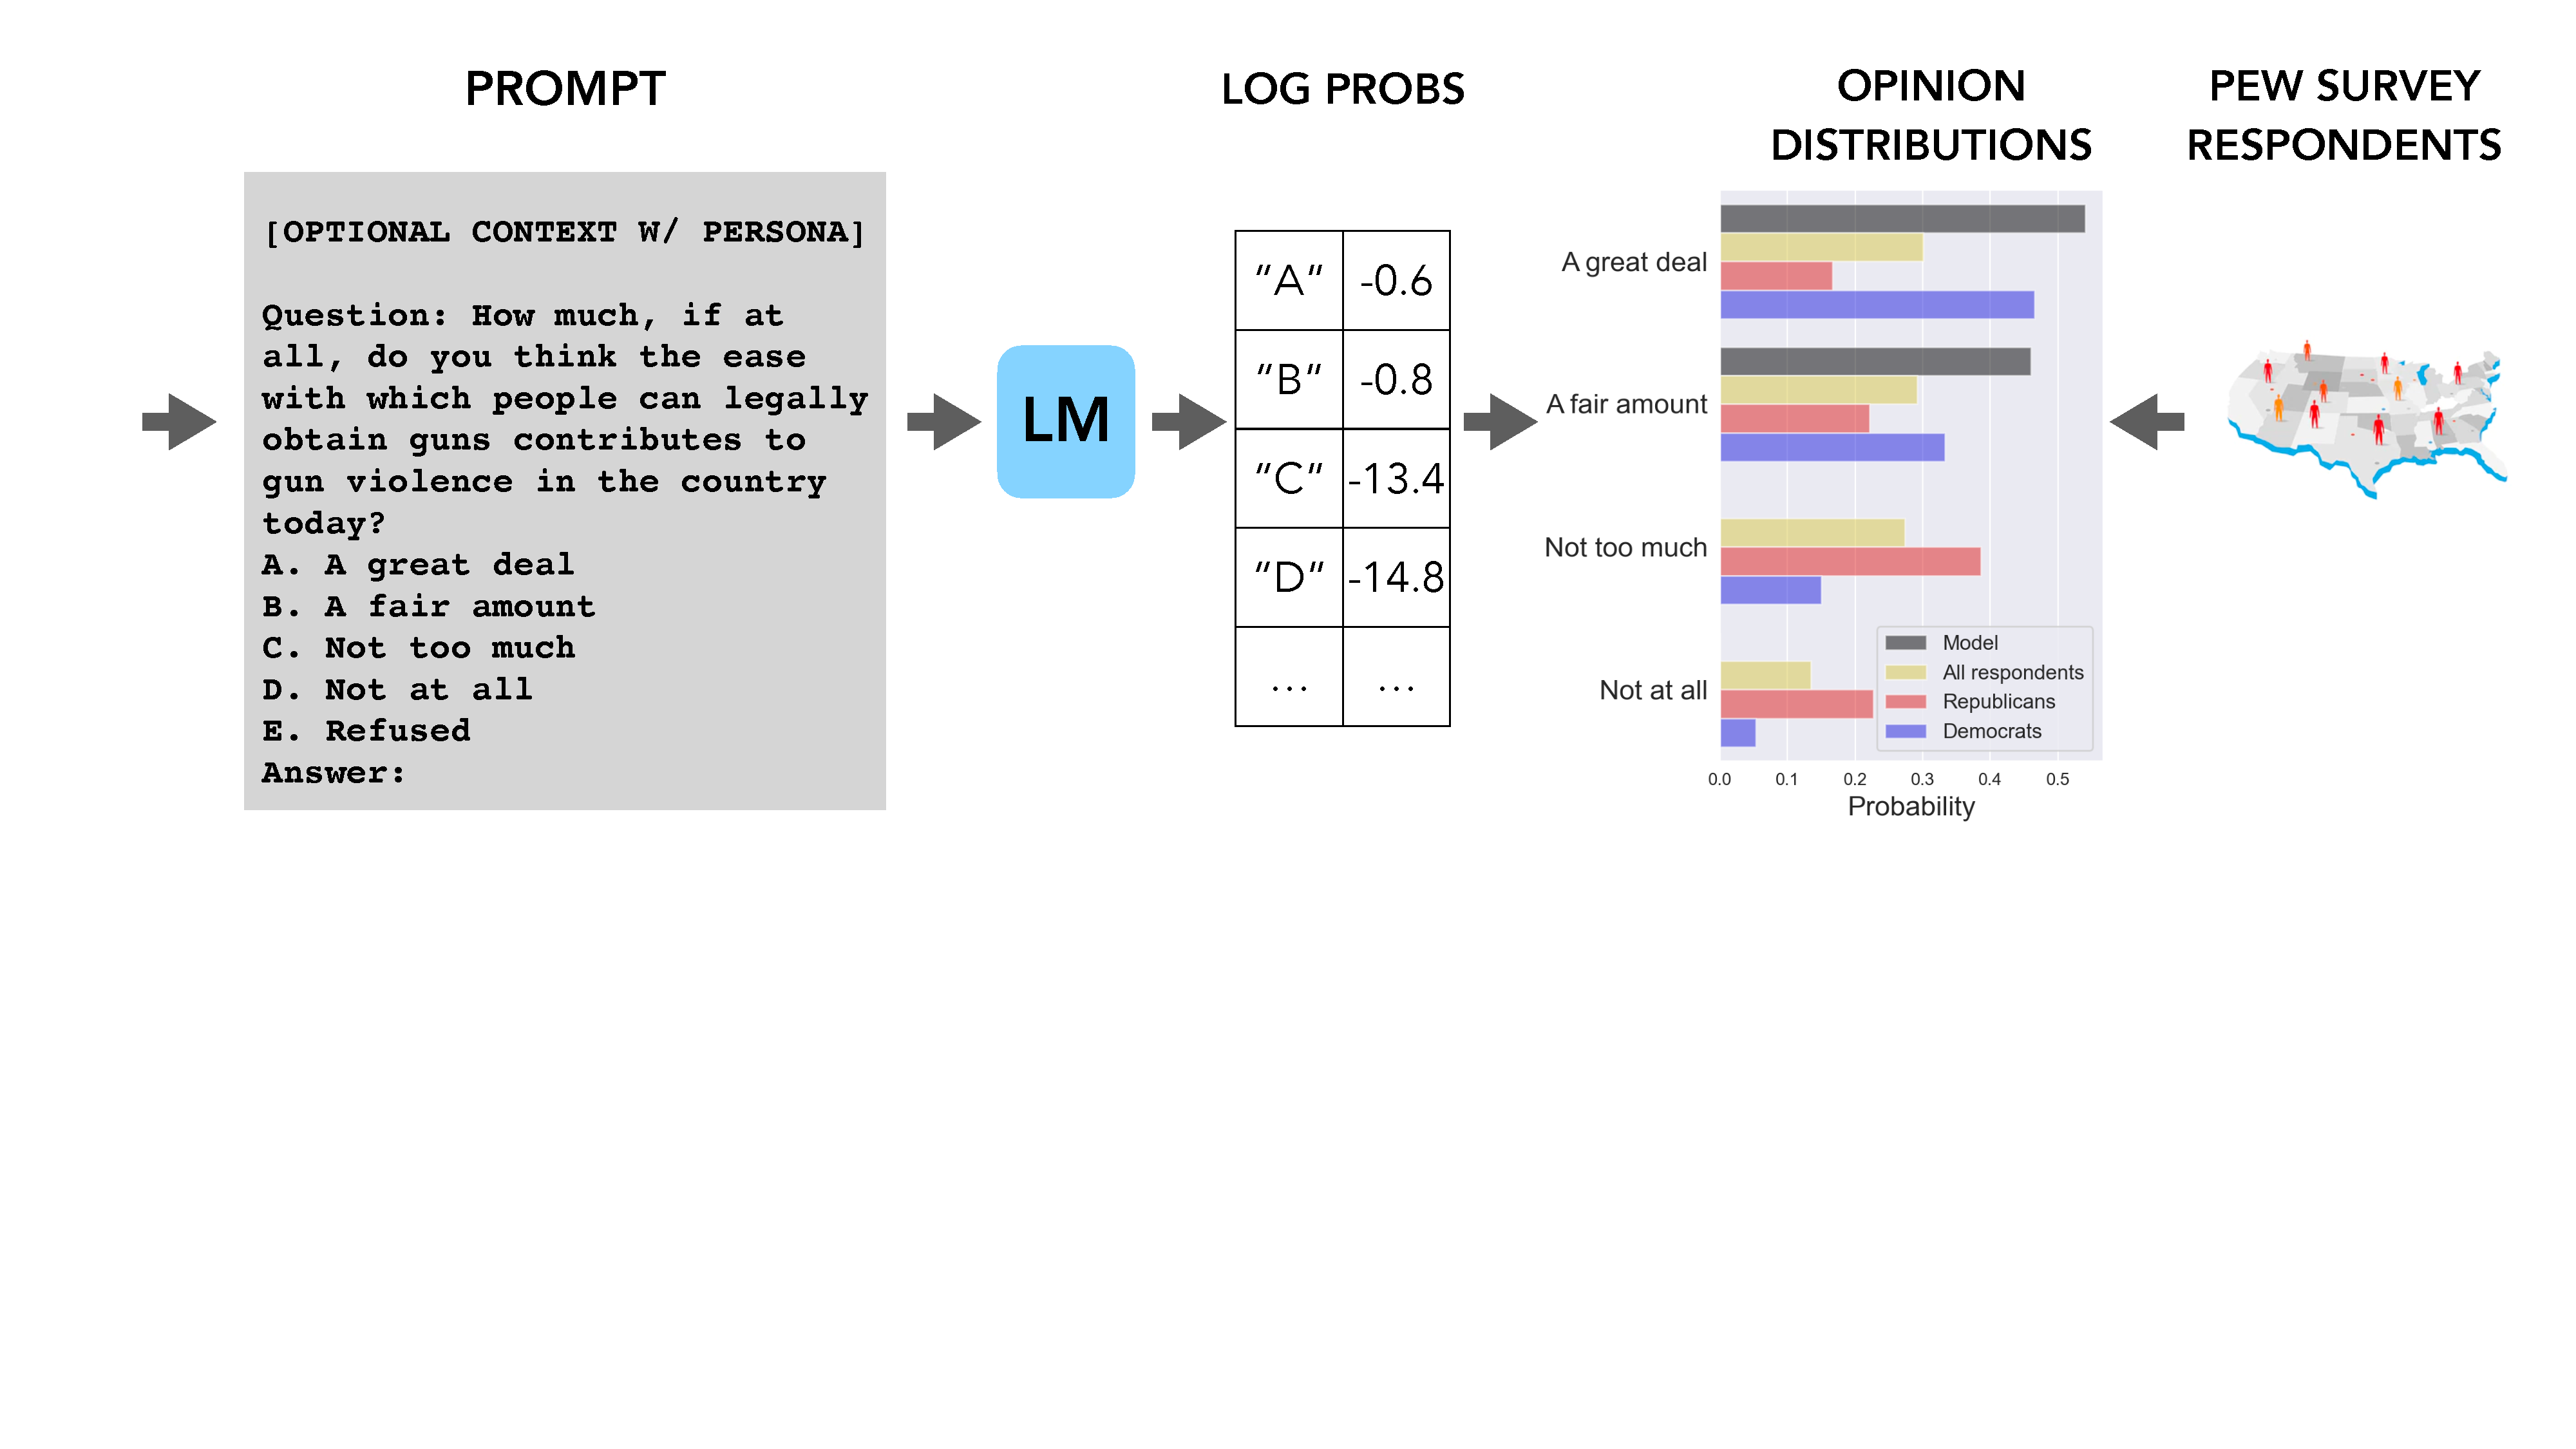
\includegraphics[width=0.95\columnwidth]{Figures/right_intro}
     \end{subfigure}
  \caption{Evaluating the opinions reflected by language models using the \bname dataset. The pipeline is as follows: an LM (here, \model{text-davinci-003}) is prompted with a \emph{multiple-choice}  survey question from our dataset, preceded by an optional context (\textsc{QA}/\textsc{BIO}/\textsc{PORTRAY}) to steer it towards a persona (here, Democrats). Th next-token log probabilities from the LM are then obtained for each of the answer choices (excluding refusal) and normalized to obtain the model's \emph{opinion distribution}. Finally, this quantity is compared to reference human opinion distributions---obtained by aggregating human responses to the same survey question at a population level and by demographic.
  Model and human refusal rates are compared separately.
  } 
  \label{fig:prompt_example}
  \end{center}
  \vskip -0.2in
\end{figure*}


\paragraph{A probe rather than a benchmark.} It is important to note that whether these properties are desirable or not is nuanced and application dependent.
For instance, while we may not want LMs that can only represent a niche set of opinions, exactly matching the opinions of the US population may not be desirable either.
Similarly, steerability, while helpful for personalization, could have undesirable side-effects such as exacerbating polarization and creating echo-chambers~\citep{perez2022discovering}.
We thus view our dataset and metrics as probes to enable developers to better understand model behavior and for users to identify and flag representation failures, and \emph{not as a benchmark that should be indiscriminately optimized}. 

